\chapter{Encapsulation}


	\section{Introduction}

	The extendability of the feature library is based on the concept of
	{\em Encapsulation}.
	A large number of components that are manufactured start with the raw 
	material as a rectangular block. The goal of process planning is to start 
	from this rectangular shape and produce the final shape. 
	{\em Orthohedral encapsulation } was thus a natural choice to start with. 
	Bar stocks are also very common, but they usually restrict the final shape 
	to parts with rotational geometry. This {\em Cylindrical 
	Encapsulation} is not directly dealt with in the present work, but can
	be treated as a special case of orthohedral encapsulation.

	This chapter describes how the concept of {\em Encapsulation} has been 
	implemented in the current feature based design system. The process of 
	extending the feature library is explained with an example. Finally,
	it is shown how components with free form surfaces can be modeled using
	the idea of encapsulated blocks in conjunction with a B-Spline surface.

	\section{Basics}

	Mechanical components come in a wide variety of shapes and sizes. To 
	bring them all within the realm of solid modeling in exact form is not 
	an easy task. Limitations imposed by the lack of an adequate mathematical 
	description, computational power and human power
	makes it necessary to idealize them. The present system has implemented
	shapes with a relatively simple mathematical description. Still, it 
	is not a simple matter
	to define operations and connectivities in terms of individual shapes.
	A layer is needed to hide aspects of the shape geometry 
	which are not relevant to a particular operation and give only those
	that are necessary.  This ``hiding'' of the true shape is called 
	``Encapsulation''.

		Encapsulation divides the real shape into two parts :


		\begin{enumerate}
		\item
		External shape, which gives an idealized external geometry which
		encloses the true shape.
		\item
		Internal shape, which defines the actual geometry of the shape.
		\end{enumerate}

	The definition of a mapping between the external shape and the internal 
	shape is necessary for the definition of the encapsulated geometry.
	The encapsulated block may require some more parameters which may be
	requested from the user. The user needs to define operations for the
	encapsulated block which fall into the following categories :
		\begin{enumerate}
		\item
		{\em No-Change functions}, which are the same as the function
		developed for the external shape. e.g., addition or the
		deletion of the block from a component.
		\item
		{\em New functions}, which are specific to the internal shape and
		are not relevant for the external shape, e.g., the user input
		of control points for a B-Spline surface.
		\item
		{\em Overwritten functions}, which overwrite the corresponding 
		external shape function completely, e.g., the display function.
		\item
		{\em Add-on functions}, which add a function to the corresponding
		external shape function, e.g., the create function.
		\end{enumerate}

	In our work, the external shape for all blocks is a rectangular 
	parallelopiped with orthohedral geometry.
	The definition of internal shape is different for different encapsulated
	block types as described below :
    \begin{enumerate}

    \item
    Constructive block (ADDTblock)

        \begin{figure}[htbp]
            %\centerline{\psfig{figure=addblk.ps,width=2.0in,height=2.0in}}
            \hspace{4cm}
            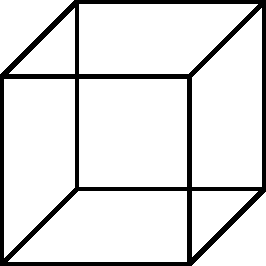
\includegraphics[width=2.0in,height=2.0in]{ADDBLK.pdf}
            \caption{Constructive Block}
            \label{addblk}
        \end{figure}

        A constructive block feature (Figure ~\ref{addblk}) is a feature
        with six bounding faces
        where each face is perpendicular to one of the coordinate axes. In this
        case the internal shape is geometrically identical to the external 
		shape. No additional parameters are necessary to define the geometry.

    \item
    Subtractive block  (SUBTblock)

        \begin{figure}[htbp]
           % \centerline{\psfig{figure=subblk.ps,width=2.0in,height=2.0in}}
            \hspace{4cm}           
           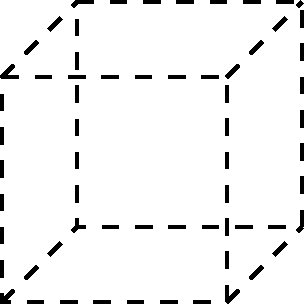
\includegraphics[width=2.0in,height=2.0in]{SUBBLK.pdf}
            \caption{Subtractive block}
            \label{subblk}
        \end{figure}

        A subtractive block (Figure ~\ref{subblk}) is geometrically identical
        to a constructive block, but physically it represents a
        negative volume. The order of the vertices in each face is the reverse 
		of that in the faces of a constructive block.

    \item
    Constructive cylinder (ADDTcyl)
	
	        \begin{figure}[htbp]
	        %    \centerline{\psfig{figure=addcyl.ps,width=2.0in,height=2.0in}}
            \hspace{4cm}	        
	        \includegraphics[width=2.0in,height=2.0in]{ADDCYl.pdf}
	            \caption{Constructive Cylinder}
	            \label{addcyl}
	        \end{figure}
        A constructive cylinder (Figure ~\ref{addcyl}) is 
        enclosed in an external rectangular block. The axis of the cylinder 
		needs
        to be specified as an additional parameter. The lengths in the other two
        directions determine the major and minor diameters of the cylinder. If
        they are different, an elliptical cylinder is constructed.

    \item
    Subtractive cylinder (SUBTcyl)

        \begin{figure}[htbp]
          %  \centerline{\psfig{figure=subcyl.ps,width=2.0in,height=2.0in}}
                      \hspace{4cm}
          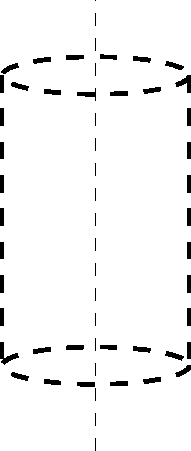
\includegraphics[width=2.0in,height=2.0in]{SUBCYL.pdf}
            \caption{Subtractive Cylinder}
            \label{subcyl}
        \end{figure}

        A subtractive cylinder (Figure ~\ref{subcyl}) is geometrically
        similar to a constructive cylinder. It differs
        only in the face orientations and represents a hole.

    \item
    Constructive wedge (ADDTwedge)

        \begin{figure}[htbp]
          %  \centerline{\psfig{figure=addwed.ps,width=2.0in,height=2.0in}}
                      \hspace{4cm}
          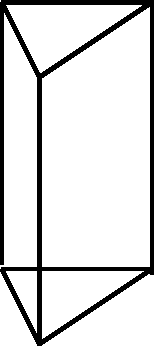
\includegraphics[width=2.0in,height=2.0in]{ADDWED.pdf}
            \caption{Constructive Wedge}
            \label{addwed}
        \end{figure}

        A constructive wedge (Figure ~\ref{addwed}) is modeled as
        a right angled triangular prismatic block enclosed in the external
        shape. The user needs to specify the axis and the two butting
        planes.

    \item
    Subtractive wedge (SUBTwedge)

        \begin{figure}[htbp]
         %   \centerline{\psfig{figure=subwed.ps,width=2.0in,height=2.0in}}
                     \hspace{4cm}
         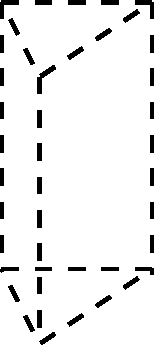
\includegraphics[width=2.0in,height=2.0in]{SUBWED.pdf}
            \caption{Subtractive Wedge}
            \label{subwed}
        \end{figure}

        A subtractive wedge (Figure ~\ref{subwed}) is geometrically identical
		to the constructive wedge but differs in the orientation of the
        faces.

    \item
    Constructive B-spline (ADDTbspline)

        \begin{figure}[htbp]
         %   \centerline{\psfig{figure=addbsp.ps,width=3.0in,height=2.0in}}
                     \hspace{4cm}
         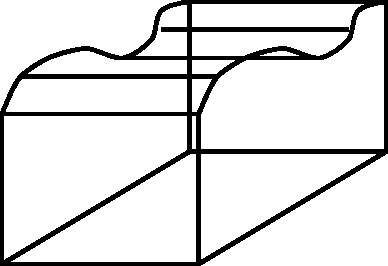
\includegraphics[width=3.0in,height=2.0in]{ADDBSP.pdf}
            \caption{Constructive B-spline}
            \label{addbsp}

        \end{figure}

        A constructive B-spline represents a block in which one surface is an
		extruded B-spline surface. Apart
        from the external block information, the user needs to specify an axis 
		for extrusion and the control points to define the B-spline.

    \end{enumerate}

	\section{Advantages of Encapsulation}
		\begin{enumerate}
			\item
			It provides a mechanism to extend and customize the shape library
			\item
			It allows handling of complex geometry while maintaining simplicity
			of the block structure.
			\item
			It simplifies addition of a new shape as the functionality related
			to the external shape such as ``Create'',``Edit'', etc. are
			already developed. The user needs to code only those functions
			which are related to internal geometry such as ``local edit'',
			``polygon-set display'', etc.
		\end{enumerate}
	\section{Extension of the Feature Library}

		A rich feature library is a prime requirement of a feature-based 
		modeling
	system. In addition, it should be possible to extend it depending
	on the family of parts to be modeled. This capability is provided
	in the current prototype feature based design system. To illustrate how 
	this is done, the development of a right-angled wedge feature is presented 
	in detail below. The feature is developed starting with the basic 
	rectangular block which encapsulates it and going through the following 
	steps :
	\begin{enumerate}
	\item
	Once the external rectangular block has been specified, the additional 
	information required to define the wedge consists of :

		\begin{itemize}
		\item
		Axis of the wedge. The planes perpendicular to this axis
		are defined as the ``top'' and the ``bottom'' planes.
		\item
		Two butting planes. These are the rectangular faces of the wedge that
		are perpendicular to each other (Fig. ~\ref{wedblk}	).
		\end{itemize}

		\begin{figure}[htbp]
		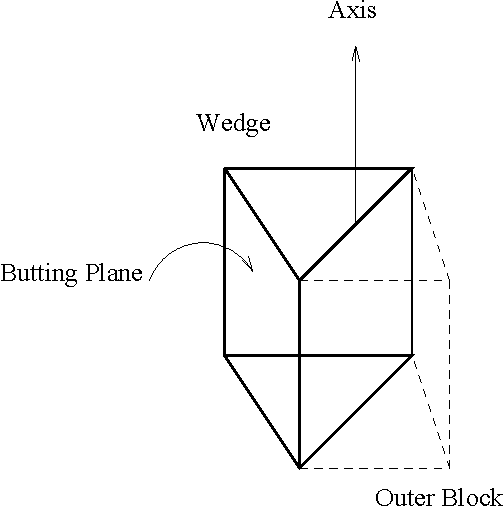
\includegraphics[scale=1.2]{WEDBLK.pdf}
	            \caption{Constructive Wedge encapsulated in Block}
	            \label{wedblk}
  		\end{figure}

	\item
	Definition of Operations :

		\begin{itemize}
		\item
		{\em Create-Polygons()} : This function returns a list of the polygons 
		consisting
		of three side faces and two triangular faces representing the top
		and the bottom of the wedge. This function replaces the functionality
		developed for the external shape.

		\item
		{\em Display()} :
		The {\em Display} function first calls the {\em Create-Polygons} 
		function. Polygons that are
		displayed have two triangles (representing top and bottom ) and
		three rectangular polygons (representing sides). This function
		overwrites the display functionality developed in the parent classes.
		\item
		{\em Create()} : The {\em Create} functionality adds the user input 
		procedure for the additional data members defined for the wedge.
		\item
		{\em Add-Block()} : Addition of the wedge is the same as an 
		addition of the external shape.
		\end{itemize}
	\end{enumerate}

    \section{Swept B-spline Encapsulated Block}

	A B-Spline surface feature is provided to allow the user to model 
	free-form surfaces.
	The idea of encapsulation is used to model this relatively complex shape,
	while still exploiting the simplicity offered by the generalized orthohedral
	block structure. Most of the functionality defined for the external shape
	remains valid for the B-spline block also. This reduces the number of 
	operations that need to be implemented separately for the B-spline block.
	A local coordinate system is
	developed within the external shape and is used to define the mapping 
	between the external rectangular shape
	and the internal B-Spline geometry. The mapping is defined as follows :
		\begin{itemize}
		\item
		The
		axis of the B-spline block is defined as the axis along which a B-spline
		curve is extruded (i.e. swept). 
		\item
		The extrusion is confined between the 
		MIN and the MAX of the external block along the axis of the B-spline.
		\item
		B-spline curve is defined in the plane normal to the axis of the
		B-spline block. For example, if the axis of the B-spline block is
		in the Z direction then the B-spline curve is defined in the X-Y plane.
		\item
		Definition of the B-spline curve	requires following parameters :

            \begin{enumerate}
            \item
            Order of the B-spline
            \item
            Knot vector
            \item
            Control Points
            \end{enumerate}

		\item
		The control points are defined in a local normalized coordinate system, 		in which coordinate varies from 0 to 1 over the block.

		\item
		The Bounds of the B-spline curve along the coordinate directions
		perpendicular to its axis correspond to the MIN and
		the MAX of the external block in the respective direction. For example,
		consider a B-spline block along the Z-axis. The $x$ and $y$ values 
		of the control points range between 0 to 1, where ``0'' gets mapped to 
		the MIN and ``1'' gets mapped to the MAX in both directions.

		\item
		As the B-spline surface is defined relative to the external shape, any
		change in the external shape gets reflected correspondingly to the
		absolute positioning of the control vertices; however their values in
		the local coordinate system remain unchanged.

		\end{itemize}

    \subsection{Operations}

        \begin{itemize}
        \item
        {\em Create()} : The Create functionality adds the user input procedure
        for the additional data members defined for the {\em B-spline}.
		The current implementation has limited the number of control
		points to twenty. The user first inputs the external shape data and
		the axis of the B-spline surface. The default control points are
		calculated internally as follows :
			\begin{itemize}
			\item
			The user is prompted to choose the axis of the B-spline block.
			\item
			A plane whose normal lies along the axis of the B-spline is selected
			for the curve definition. For example, if the user selects Z axis
			as the axis of the B-spline then Z-MAX plane is selected for the
			curve definition.

			\item
			The MIN and the MAX values are retrieved from the external block
			geometry for the next direction (in cyclic order : X 
			$\rightarrow$ Y $\rightarrow$ Z) to the axis of the B-spline block.
			Thus, in the example considered in the previous step, a default
			2D curve is presented to the  user with $x$ values equally spaced
			between X-MIN and X-MAX, while $y$ values are constant at Y-MID.

			\item
			The user is allowed to change the values of these points to model
			the B-spline curve, after which extrusion is done to generate the 
			B-spline surface.
			\end{itemize}


        \item
        {\em Add-Block()} : Addition of a {\em B-spline} block is the same as 
		the addition of the external shape. The B-spline does not change this
		function of a {\em Block}. It is assumed that the user,
		while specifying the topological link with the B-spline, chooses a
		plane surface of the B-spline block as the resting plane.
		
		\item
		{\em Edit()} : Modification of the external shape changes the overall 
		size, shape, 
		and location of the block in the component. The procedure for 
		modification of the
		external shape parameters is not changed by the B-spline block. 
		Thus, if the external shape is reduced/enlarged, the B-spline block
		also gets correspondingly reduced/enlarged. This is possible because
		the control points of the B-spline are defined relative to the shape
		of the external block. The user may be given an option of editing the
		B-spline block in the absolute coordinate system. The 
		B-spline block
		adds functionality to the local edit, where modification of the
		positions of the
		control points is performed. The local edit of the B-spline surface is 
		proposed as follows :

			\begin{itemize}
			\item
			The user is presented with the list of control point values.
			\item
			The user is allowed to change the coordinates.
			\item
			It is assumed that the user does not change the values such that 
			the surface interfaces with other blocks in the component; this
			can be done by placing all the control points inside the external
			shape.
			\end{itemize}

		\item
		\label{genpts}
		{\em Dimensioning} : The dimensioning scheme formulation requires
		contribution of the dimensioning planes from individual blocks. The
		dimensioning planes should completely specify the internal shape of the
		block. Refer section ~\ref{dimpts} for further details. 

		\item
        {\em Display()} :
        The Display function 
        overwrites the display function of the parent classes and
		displays the B-Spline surface. The NURB \footnote{ Non-Uniform Rational
		B-spline} surface primitive of PHIGS is used to display the B-spline
		surface. Although a polygon-set display facility has not yet been
		implemented, it would be done by generating a grid of points on the
		surface and approximating the surface by a set of rectangular faces
		on its grid.

        \end{itemize}

